\documentclass[11pt, a4paper]{article}
\usepackage{microtype}
\usepackage{amsmath}
\usepackage{amssymb}
\usepackage{booktabs}
\usepackage{array}
\usepackage[margin=1in]{geometry} % set page margins automatically
\usepackage{siunitx}
\usepackage{graphicx}
\usepackage{lmodern}  % better i18n Postscript version of Knuth's cm fonts
\usepackage{url}
\usepackage[parfill]{parskip}
\usepackage[T1]{fontenc}
\usepackage[italian]{babel}
\usepackage[print-unity-mantissa=false]{siunitx}
\usepackage{chemmacros}
\usepackage[version=4]{mhchem}
\usepackage{fancyvrb}
\usepackage{hyperref}
\usepackage{graphicx}
\usepackage{float}
\usepackage[bottom]{footmisc}
\usepackage{textgreek}
\usepackage{subcaption}
\usepackage[style=authoryear-comp,url=false,maxcitenames=1,sorting=none]{biblatex}
\usepackage{csquotes}
\usepackage{caption}
\usepackage{bookmark}
\usepackage{braket}

\listfiles

\captionsetup[figure]{font=small}
\renewcommand*{\thefootnote}{(\arabic{footnote})}

\DeclareCiteCommand{\supercite}[\mkbibsuperscript]
  {\iffieldundef{prenote}
     {}
     {\BibliographyWarning{Ignoring prenote argument}}%
   \iffieldundef{postnote}
     {}
     {\BibliographyWarning{Ignoring postnote argument}}}
  {\usebibmacro{citeindex}%
   \bibopenbracket\usebibmacro{cite}\bibclosebracket}
  {\supercitedelim}
  {}

\DeclareMathOperator{\Tr}{Tr}

\addbibresource{creutz.bib}

\begin{document}


\title{\vspace{-6em}\huge{Approccio statistico all'oscillatore (an)armonico quantistico}\vspace{-2ex}}
\author{Gianluca Zappavigna}
\maketitle

\section{Introduzione}

Riformulando l'evoluzione temporale in meccanica quantistica in termini di integrali di cammino, riusciamo ad esprimere il problema in una forma che possiamo interpretare in maniera probabilistica, e quindi a trattare numericamente con un metodo Monte Carlo.

Consideriamo la funzione di Green

\begin{equation}
  \Braket{q',t' | q,t} = \Braket{q' | e^{-iH(t'-t)} | q} = \Braket{q' | e^{-H(\tau'-\tau)} | q}
\end{equation}

dove $t = -i \tau$ e $t' = -i \tau'$. Possiamo riscrivere l'operatore di evoluzione temporale da $\tau$ a $\tau'$ come la composizione di N operatori analoghi,
dove ciascuno fa evolvere la funzione d'onda di un passetto lungo $a$.

\begin{equation}
  \Braket{q' | e^{-H(\tau'-\tau)} | q} = \Braket{q' | \underbrace{e^{-Ha} e^{-Ha} \ldots e^{-Ha}}_{n \text{ volte}} | q}
\end{equation}

Ammettendo che l'Hamiltoniana sia della forma $H(q, p) =  \frac{1}{2} \sum_{\alpha=1}^{n} p_{\alpha}^2 + V(q)$, possiamo riscrivere, attraverso una serie di calcoli (un po' laboriosi..), la funzione di Green nel seguente modo

\begin{equation}
  \label{green2}
  \Braket{q' | e^{-iH(t'-t)} | q} \approx \int \prod_{l'=1}^{N-1} \prod_{\alpha=1}^n \frac{dq_{\alpha}^{(l')}}{\sqrt{2 \pi a}} e^{-\sum_{l=0}^{N-1} a L_E(q^{(l)}, \dot{q}^{(l)})}
\end{equation}
dove $L_E(q^{(l)}, \dot{q}^{(l)})$ vale

\begin{equation}
  L_E(q^{(l)}, \dot{q}^{(l)}) = \frac{1}{2}\sum_{\alpha} \left[\dot{q}_{\alpha}^{(l)}\right]^2 + V(q^{(l)})
  = \frac{1}{2}\sum_{\alpha} \left[\frac{q_{\alpha}^{(l+1)} - q_{\alpha}^{(l)}}{a}\right]^2 + V(q^{(l)})
\end{equation}

Questa formula non è esatta perché nella derivazione è stata fatta la prima fondamentale approssimazione: data la forma assunta di $H(q, p)$, si è sfruttata la formula di Baker-Campbell-Hausdorff (troncata al primo ordine della serie) per ottenere:

\begin{equation}
  e^{-Ha} = e^{- a \frac{1}{2} \sum_{\alpha=1}^{n} p_{\alpha}^2 - a V(q)} \approx e^{- a \frac{1}{2} \sum_{\alpha=1}^{n} p_{\alpha}^2} e^{-a V(q)}
\end{equation}

Questo implica che l'accuratezza della relazione che abbiamo ottenuto dipende dalla lunghezza dell'intervallo $a$.
Si noti che in \eqref{green2} l'argomento dell'esponenziale ha l'aspetto di un'azione discretizzata, cioè equivale a una stima numerica dell'integrale della Lagrangiana lungo un cammino.
Possiamo pensare che l'integrale che abbiamo ottenuto sia un integrale su tutti i possibili cammini.
Si tratta però di cammini ``discretizzati'', per i quali ciascun passo corrisponde ad un intervallo temporale $a$.

L'integrale ottenuto può essere riconosciuto nella forma:

\begin{equation}
  \label{prob_distr}
  \Braket{q' | e^{-iH(t'-t)} | q} \approx \int_{q}^{q'} Dq\, e^{-S_E[q]}
\end{equation}

Allora $e^{-S_E[q]}$ può essere visto come il peso statistico che quantifica il contributo di ciascun cammino nella somma.
Se ora facciamo coincidere lo stato di partenza con quello di arrivo ($q' = q$), cioè consideriamo solo cammini chiusi, e integriamo su tutti gli stati di partenza (e quindi di arrivo) $q$, otteniamo un'espressione che formalmente rappresenta una funzione di partizione:

\begin{equation}
  \int dq \Braket{q | e^{-iH(t'-t)} | q} = \Tr(e^{-iH(t'-t)}) = \Tr(e^{-iHT}) = Z
\end{equation}

dove si è introdotto $T = t'-t$, che rappresenta il periodo del cammino.
Nota la funzione di partizione, significa che siamo in grado di calcolare il valore d'aspettazione di un osservabile $A$.

\begin{equation}
  \left\langle A \right\rangle = \frac{\Tr\left(A \, e^{-HT}\right)}{\Tr\left(e^{-HT}\right)}
\end{equation}

Esprimendo la traccia in termini della base formata dagli autostati dell'energia, ci accorgiamo di una proprietà interessante:

\begin{equation}
  \left\langle A \right\rangle =
  \frac{\Tr\left(A \, e^{-HT}\right)}{\Tr\left(e^{-HT}\right)} =
  \frac{\sum_{n} \Braket{n | A e^{-H T} | n} }{\sum_{n} \Braket{n | e^{-H T} | n}} =
  \frac{\sum_{n} e^{-E_n T} \Braket{n | A | n}}{\sum_{n} e^{-E_n T}} =
\end{equation}

Per $T \to \infty$, il fattore esponenziale dominante è quello corrispondente all'autovalore più piccolo, cioè $E_0$. Allora scopriamo che

\begin{equation}
  \label{proj_void}
  \left\langle A \right\rangle =
  \frac{\sum_{n} e^{-E_n T} \Braket{n | A | n}}{\sum_{n} e^{-E_n T}} \xrightarrow[T \to \infty]{} \Braket{0 | A | 0}
\end{equation}

Quindi, se il periodo dei cammini che consideriamo è sufficientemente lungo, possiamo ottenere una stima della cosiddetta ``proiezione sul vuoto'' dell'operatore $A$
se siamo in grado di calcolare il suo valor medio.

In conclusione, per arrivare ad una buona stima, abbiamo due prescrizioni a cui dobbiamo prestare attenzione: $a$ deve esse sufficientemente piccolo e $T$ deve essere sufficientemente grande.
Siccome $T$ sarà necessariamente un multiplo di $a$, conviene fin da subito far riferimento al numero di passi $N = T / a$.

Possiamo allora cercare di campionare numericamente dei possibili cammini, secondo la distribuzione definita sopra, per ottenere informazioni su un dato sistema.
Ma quale algoritmo usare? E quale sistema studiare?


\subsection{Hybrid Monte Carlo}

L'algoritmo scelto per campionare la distribuzione dei cammini è \emph{Hybrid Monte Carlo}. Questo algoritmo fa parte della famiglia di metodi noti come Markov Chain Monte Carlo (MCMC).
L'elemento comune a tutti questi metodi è che campionano una certa distribuzione di probabilità costruendo una catena di Markov tale da avere come distribuzione stazionaria proprio la distribuzione prescelta.
Questo algoritmo è anche detto \emph{Hamiltonian Monte Carlo}, poiché un elemento chiave dell'algoritmo richiede di far evolvere un sistema Hamiltoniano attraverso le equazioni del moto che ne derivano.
L'Hamiltoniana di questo sistema non è quella del sistema da cui siamo partiti, ma è quella associata ad un nuovo problema ``fittizio''.


\begin{equation}
  \mathcal{H}[\{\phi_i, \pi_i\}] = \sum_{i} \frac{\pi_i^2}{2} + S[\{\phi_i\}]
\end{equation}

Qui le $\phi_i$ giocano il ruolo delle $q_i$ nella discussione precedente. L'elemento nuovo, che non ha nessun legame con il sistema fisico che vogliamo studiare, sono le $\pi_i$.
Introdurre queste variabili ci serve solo nell'implementazione di Hybrid Monte Carlo.
\`E chiaro però dalla loro forma che rappresentano dei momenti.

I passi prescritti dall'algoritmo sono mostrati di seguito. Questi passaggi vengono iterati, e ognuno produce un singolo campione della distribuzione.

\begin{enumerate}
  \item Estrarre ${\pi_i}$ secondo una distribuzione Gaussiana, cioè
  \begin{equation}
    P(\{\pi_i\}) = \left(\prod_i \frac{1}{\sqrt{2 \pi}}\right) e^{-\sum_i \frac{\pi_i^2}{2}}
  \end{equation}
  \item Far evolvere il sistema, partendo dallo stato $\{\phi_i, \pi_i\}$, secondo le equazioni di Hamilton
  \begin{equation}
    \begin{cases}
      \dot{\phi}_k = \frac{\partial \mathcal{H}}{\partial \pi_k} = \pi_k \\
      \dot{\pi}_k = -\frac{\partial \mathcal{H}}{\partial \phi_k} = -\frac{\partial S}{\partial \phi_k} \\
    \end{cases}
  \end{equation}
  di un tempo $T_\text{HMC}$, per arrivare allo stato $\{\phi'_i, \pi'_i\}$.
  \item $\{\pi'_i\}$ rappresenta il candidato per il campione successivo dell'iterazione. Viene accettato però con probabilità
  \begin{equation}
    P_A \left(\{\phi_i, \pi_i\} \rightarrow \{\phi'_i, \pi'_i\} \right) = \min\left\{1,\, e^{\mathcal{H}[\{\phi'_i, \pi'_i\}] - \mathcal{H}[\{\phi_i, \pi_i\}]}\right\}.
  \end{equation}
  Se il candidato non viene accettato, il nuovo campione rimane $\{\phi_i\}$.
  \item I momenti $\{\pi_i\}$ e $\{\pi'_i\}$ vengono ignorati e l'iterazione riparte dal punto 1.
\end{enumerate}

Per risolvere numericamente le equazioni scegliamo di usare il metodo di integrazione \emph{leapfrog}.
Quindi dovremo scegliere due parametri, puramente tecnici: il passo di integrazione $\Delta t$ e il numero di passi $N_{\text{HMC}}$, tali che $N_{\text{HMC}} \cdot \Delta t = T_\text{HMC}$.

Il punto 3 è la stessa regola che si incontra nell'algoritmo di Metropolis, e ha lo scopo di garantire che l'equazione del bilancio dettagliato sia rispettata.
Ricordiamo che il bilancio dettagliato è una condizione sufficiente, ma non necessaria, affinché la distribuzione stazionaria della catena di Markov coincida con quella desiderata.

Nel dimostrare che questa proprietà è soddisfatta si assume la reversibilità delle equazioni di Hamilton.
Lo schema di integrazione scelto (leapfrog) è simplettico, il che garantisce la reversibilità temporale.
Questa proprietà però è vera solo in linea teorica. Nella realtà dobbiamo fare i conti con gli errori di round-off. Questo significa che dovremo verificare che leapfrog sia sufficientemente accurato sotto questo punto di vista.
Quello che faremo sarà ripetere a ritroso la traiettoria ottenuta dall'integrazione, invertendo la direzione dei momenti finali (ossia $\{\pi'_i\} \mapsto \{-\pi'_i\}$) e ripetendo lo stesso numero di passi $N_{\text{HMC}}$ di lunghezza $\Delta t$.
Se la posizione $\{\phi^{\text{(rev)}}_i\}$ che otteniamo si trova entro una certa soglia dalla posizione iniziale $\{\phi_i\}$, allora consideriamo la soluzione numerica accettabile.

Nel caso questa condizione non fosse verificata è necessario calibrare i parametri che determinano la traiettoria calcolata dall'integrazione numerica, $\Delta t$ e $N_{\text{HMC}}$.

\subsection{Oscillatore armonico quantistico}

Il sistema fisico a cui vogliamo applicare la metodologia discussa fin'ora è l'oscillatore armonico quantistico. La sua Hamiltoniana è data da
\begin{equation}
  H = \frac{\hat{p}^2}{2m} + \frac{1}{2} m \omega^2 \hat{x}^2
\end{equation}

La corrispondente azione discretizzata $S_E$, che compare nella formula \eqref{prob_distr}, diventa

\begin{equation}
  S = \sum_{j=1}^N a \left[
    \frac{1}{2} m \frac{\left(x_{j+1} - x_{j}\right)^2}{a^2} +
    \frac{1}{2} m \omega ^ 2 x_j^2
  \right]
\end{equation}

Per tentare di dedurre alcuni elementi salienti del sistema dai risultati numerici che otterremo, possiamo innanzitutto sfruttare la
\eqref{proj_void} per stimare l'energia dello stato fondamentale $E_0 = \Braket{0 | H | 0}$.
Ma come possiamo stimare il valor medio $\langle H \rangle$? Dopotutto, HMC ci fornisce una popolazione di cammini, quindi non esiste un modo immediato di stimare il termine cinetico $T = \frac{\hat{p}^2}{2m}$.
Per stimare $T$ ci viene in aiuto il teorema del viriale, grazie al quale sappiamo che

\begin{equation}
  \left\langle T \right\rangle =
  \left\langle \frac{1}{2} x V'(x) \right\rangle
\end{equation}

che nel caso dell'oscillatore armonico diventa

\begin{equation}
  \left\langle T \right\rangle = \left\langle \frac{1}{2} m \omega^2 x^2 \right\rangle
\end{equation}

Questa relazione ci permette di esprimere $\langle H \rangle$ esclusivamente in termini dell'operatore di posizione, ovvero

\begin{equation}
  \left\langle H \right\rangle =  \left\langle T + V \right\rangle =  \left\langle  m \omega^2 x^2 \right\rangle
\end{equation}

Esiste poi un'altra proprietà, attraverso la quale siamo in grado di stimare anche l'intervallo tra le energie dei primi due autostati di $H$, $\Delta E = E_1 - E_0$.
Consideriamo l'operatore $A = \hat{x}(\tau) \hat{x}(0)$, dove utilizziamo la rappresentazione di Heisenberg, in cui sono gli operatori (e non gli stati), ad evolvere.
$\hat{x}(\tau)$ è quindi pari a $e^{H \tau} \hat{x} e^{-H \tau}$ (stiamo ancora utilizzando il tempo immaginario).

\begin{align}
  \Braket{0 | \hat{x}(\tau) \hat{x}(0) | 0} = \Braket{0 | e^{H \tau} \hat{x} e^{-H \tau} \hat{x} | 0} = \\
  \sum_{n} \Braket{0 | e^{H \tau} \hat{x} e^{-H \tau} | n} \Braket{n | \hat{x} | 0} = \\
  \sum_{n}  e^{-\left(E_n - E_0\right) \tau} \Braket{0 | \hat{x}  | n} \Braket{n | \hat{x} | 0} = \\
  \sum_{n}  e^{-\left(E_n - E_0\right) \tau} \left| \Braket{0 | \hat{x}  | n} \right|^2  \label{deltae_prop_sum}
\end{align}

La forma dell'Hamiltoniana dell'oscillatore armonico permette di riscrivere l'operatore di posizione in termini degli operatori di creazione e distruzione.
A noi basta sapere che $\hat{x} \propto \hat{a} + \hat{a}^\dagger$ e siccome valgono le identità $\hat{a} \Ket{n} = \sqrt{n} \Ket{n - 1}$ e $\hat{a}^\dagger \Ket{n} = \sqrt{n + 1} \Ket{n + 1}$,
troviamo che l'unico termine a sopravvivere è quello per $n=1$. Infine, ciò che ne deduciamo è che vale la relazione di proporzionalità

\begin{equation}
  \label{deltae_prop}
  \Braket{0 | \hat{x}(\tau) \hat{x}(0) | 0} \propto e^{-\left(E_1 - E_0\right) \tau}
\end{equation}

Quindi, sempre facendo riferimento alla \eqref{proj_void}, possiamo stimare questa proiezione sul vuoto calcolando il valor medio $\langle \hat{x}(\tau) \hat{x}(0) \rangle$ per diversi valori di $\tau$ e poi estrapolare $E_1 - E_0$ attraverso un fit esponenziale.
Naturalmente, i valori di $\tau$ per cui ci è possibile questa stima sono dati dal set di tempi per cui i cammini sono noti (che dipendono dalla scelta di $N$ e $a$).


\subsection{Oscillatore anarmonico quantistico}

Costruendo sui risultati ottenuti per l'oscillatore armonico, possiamo tentare di calcolare le stesse quantità per un sistema leggermente più complesso: l'oscillatore anarmonico quantistico. L'Hamiltoniana che considereremo è la seguente:


\begin{equation}
  H = \frac{\hat{p}^2}{2m} + \frac{1}{2} m \omega^2 \hat{x}^2 + \lambda \left(\hat{x} - x_0\right)^2 \left(\hat{x} + x_0\right)^2
\end{equation}


L'azione $S_E$ che ne deriva è quindi:

\begin{equation}
  S_E = \sum_{j=1}^N a \left[\frac{1}{2} m \frac{\left(x_{j+1} - x_{j}\right)^2}{a^2} + \frac{1}{2} m \omega ^ 2 x_j^2 + \lambda \left(x_j - x_0\right)^2 \left(x_j + x_0\right)^2\right]
\end{equation}

Per stimare l'energia dello stato fondamentale $E_0$ di questo sistema dobbiamo aggiornare il risultato che otteniamo applicando il teorema del viriale.

\begin{equation}
  \left\langle T \right\rangle =
  \left\langle \frac{1}{2} x \hat{V'}(x) \right\rangle =
  \left\langle \frac{1}{2} m \omega^2 x^2 + 2 \lambda x^2 \left(x^2 - x_0^2\right) \right\rangle
\end{equation}

\begin{equation}
  \left\langle H \right\rangle = \left\langle T + V \right\rangle =
   m \omega^2 x^2 + \lambda x^2 \left(3 x^2 - 2 x_0^2\right)
\end{equation}

Tuttavia, la relazione di proporzionalità \eqref{deltae_prop} ottenuta per l'oscillatore armonico non è più valida.
Ciò deriva dal fatto che nella somma \eqref{deltae_prop_sum}, non è più solo il termine $n=1$ a dare contributo.
Infatti, se studiamo il problema dal punto di vista della teoria delle perturbazioni, e quindi consideriamo il termine quartico
la perturbazione (si assume dunque che $\lambda \ll 1$), la correzioni agli autostati contengono solo autostati con la stessa parità.
Questa proprietà discende a sua volta dalla parità di $\lambda \hat{x}^4$.
L'operatore $\hat{x}$ invece è dispari, quindi se lo applichiamo ad autostati dispari $\Ket{n}$ (con $n = 2 k + 1$), o a una combinazione lineare di questi, troviamo sempre una combinazione
di autostati pari. Risulta chiaro allora che in \eqref{deltae_prop_sum} si hanno termini non nulli per $n = 2 k + 1$.

Per tentare di stimare $\Delta E = E_1 - E_0$ per l'oscillatore anarmonico ci serve una strategia alternativa.
Prendiamo spunto da \cite{creutz_statistical_1981}, che propongono la seguente soluzione.
Partendo alla funzione di correlazione connessa a due punti

\begin{equation}
  \Gamma_c^{(2)} = \left\langle \hat{x}(\tau_1) \hat{x}(\tau_2) \right\rangle - \left\langle \hat{x}(\tau_1) \right\rangle \left\langle \hat{x}(\tau_2) \right\rangle
\end{equation}

arrivano per prima cosa allo stesso risultato già visto

\begin{equation}
  \lim_{T \to \infty} \Gamma_c^{(2)} = \Braket{0 | \hat{x}(0) \hat{x}(\tau) | 0} - \Braket{0 | \hat{x} | 0}^2 =
  \sum_{n \ne 0} e^{\frac{E_n - E_0}{\hbar} \tau} \left|\Braket{0 | \hat{x} | n}\right|^2
\end{equation}

Come discusso sopra, per $\tau \to \infty$ il termine dominante è quello per $n=1$. Se scegliamo allora un valore $\Delta \tau$ positivo si ha che

\begin{equation}
  \frac{\Gamma_c^{(2)}(\tau + \Delta \tau)}{\Gamma_c^{(2)}(\tau)} \xrightarrow[\substack{T \to \infty \\ \tau \to \infty}]{} e^{-\frac{\left(E_1 - E_0\right)}{\hbar}\Delta \tau}
\end{equation}

Quindi possiamo ottenere $E_1 - E_0$ da

\begin{equation}
  \label{creutz}
  E_1 - E_0  = \frac{\hbar}{\Delta \tau} \lim_{\substack{T \to \infty \\ \tau \to \infty}} \ln\left(\frac{\Gamma_c^{(2)}(\tau + \Delta \tau)}{\Gamma_c^{(2)}(\tau)}\right)
\end{equation}

\subsection{Equazioni di Hamilton}

Si è visto che le equazioni di Hamilton usate in Hybrid Monte Carlo dipendono dal particolare sistema studiato. In particolare, la dipendenza si manifesta nella derivata $\frac{\partial S}{\partial \phi_k}$.
Di seguito è riportato il risultato che si ottiene a partire dall'Hamiltoniana dell'oscillatore anarmonico. Il risultato analogo per l'oscillatore armonico si trova semplicemente per $\lambda=0$.
Innanzitutto $S_E$ vale:

\begin{equation}
  S_E = \sum_{j=1}^N \frac{1}{2} m \frac{\left(x_{j+1} - x_{j}\right)^2}{a^2} + \frac{1}{2} m \omega^2 x_j^2 + \lambda \left(x_j - x_0\right)^2 \left(x_j + x_0\right)^2
\end{equation}

La derivata invece è

\begin{equation}
  \frac{dS_E}{dx_i} = m \left(-x_{i-1} + 2 x_i - x_{i+1}\right) + m \omega ^ 2 x_i^2 + 4 \lambda x_i \left(x_i - x_0\right) \left(x_i + x_0\right)
\end{equation}

\subsection{Stima degli errori}

Per capire quanto accurate sono le nostre stime numeriche, abbiamo la necessità di calcolare anche delle incertezze associate.
Uno svantaggio dei metodi MCMC è che i campioni, essendo il prodotto di una catena di Markov, sono inevitabilmente affetti da correlazione temporale.

Come misura dell'incertezza considereremo la deviazione standard associata alla media campionaria $\sigma_{\overline{x}}$.
Generalmente questa è collegata alla deviazione standard $\sigma$ della distribuzione dalla relazione

\begin{equation}
  \sigma_{\overline{x}} = \frac{\sigma}{\sqrt{N}}
\end{equation}

dove $N$ è il numero di campioni della popolazione su cui viene calcolata la media campionaria.
Sorge però un problema quando i campioni non sono indipendenti. In questo caso la formula mostrata sopra sottostima sistematicamente la deviazione standard effettiva.

Se simuliamo un processo stocastico dove le distribuzioni di probabilità evolvono secondo una matrice stocastica, ci aspettiamo che i valori $f_i$ di una generica funzione $f$ calcolata sui campioni $X_i$ siano correlati, con una funzione di correlazione
che decade esponenzialmente, ovvero $\rho(t) \sim e^{-\frac{|t|}{\tau}}$.
Qui $\rho(t)$ rappresenta la funzione di autocorrelazione normalizzata, che si ottiene come $C_{ff}(t) / C_{ff}(0)$. La funzione di autocorrelazione è definita a sua volta come

\begin{equation}
  C_{ff}(t) =  \left\langle f_i f_{i+t}\right\rangle - \left\langle f_i \right\rangle ^ 2
\end{equation}

Il tempo caratteristico $\tau$ che compare nell'esponenziale può essere interpretato come il tempo medio che bisogna attendere affinché due valori assunti da $f$ risultino privi di correlazione.
Questo tempo però dipende dalla particolare scelta di $f$. Formalmente si definisce il tempo esponenziale di autocorrelazione per $f$ come

\begin{equation}
  \tau_{\mathrm{exp},f} = \limsup_{t \to \infty} \frac{t}{-\log\left|\rho_{ff}(t)\right|}
\end{equation}

Per ottenere un tempo che non dipende da $f$ ma che rappresenta il tempo di rilassamento proprio del sistema si definisce

\begin{equation}
  \tau_{\mathrm{exp}} = \sup_{f} \tau_{\mathrm{exp},f}
\end{equation}

Quest'ultimo tempo ci dice quanto impiega la catena di Markov a ``rilassare'' o ``termalizzare'', cioè quanto tempo è necessario prima che il suo stato sia indipendente dalle condizioni iniziali.
In pratica, questo valore è difficile da stimare.


Per la varianza della media campionaria dei valori $f_i$ è possibile dimostrare la seguente relazione

\begin{equation}
  \mathrm{Var}(\overline{f}) = \frac{2}{N} \tau_{\mathrm{int},f} C_{ff}(0)
\end{equation}

dove $C_{ff}(0) = \left\langle f_i ^2 \right\rangle - \left\langle f_i \right\rangle ^ 2$ corrisponde esattamente allo stimatore classico della varianza che si applica per campioni indipendenti.
$\tau_{\mathrm{int},f}$ invece è detto \emph{tempo di correlazione integrato}, ed è definito come

\begin{equation}
  \tau_{\mathrm{int},f} = \frac{1}{2} + \sum_{t=1}^{\infty} \rho_{ff}(t)
\end{equation}

Naturalmente dal punto di vista numerico la somma sarà troncata quando $\rho_{ff}(t)$ raggiunge valori trascurabili, e questo richiede circa un tempo $\tau_{\mathrm{exp},f}$.
Una precisazione importante da ricordare quando si applica questa formula è che in essa sono implicite due assunzioni.
La prima è che il numero di campioni $N$ sia $\gg  \tau_{\mathrm{exp},f}$. La seconda invece è che la media campionaria $\overline{f}$ abbia già raggiunto il suo valore di equilibrio.
Prima di iniziare a raccogliere misure per il calcolo della correlazione, e quindi dell'errore, è pertanto necessario far prima termalizzare il sistema.


\section{Risultati numerici}

La metodologia descritta sopra è stata implementata in MATLAB. Per ottimizzare i tempi di esecuzione del ciclo principale di HMC, che non può essere parallelizzato, tutto il codice relativo all'algoritmo è stato riscritto in C++.
L'analisi dei risultati invece è stata eseguita interamente in MATLAB. Per facilitare il trasferimento di dati dall'implementazione nativa in C++ all'ambiente MATLAB, è stato sfruttato il protocollo MEX, che permette di richiamare funzioni C/C++ direttamente da MATLAB.

\subsection{Considerazioni preliminari}
La qualità dell'approssimazione di $E_0$ ed $\Delta E = E_1 - E_0$ dipende, come abbiamo visto, dai parametri $a$ e $T = N a$.
Ovviamente non ci è possibile ridurre $a$ e contemporaneamente aumentare $T$ a piacere, come vorremmo.
Per il passo temporale $a$ infatti, se scegliamo valori eccessivamente piccoli incorriamo in errori di round-off che compromettono l'accuratezza dei calcoli numerici.
Sempre riguardo a questo parametro, vi è un secondo aspetto da considerare.
Più riduciamo $a$ e più il tempo di autocorrelazione dei campioni generati da HMC aumenta.
Questo è proprio il fenomeno di ``critical slowing down'' che si osserva quando si applicano metodi Monte Carlo a sistemi in condizioni prossime ad un punto critico.
Nel problema che abbiamo definito, $a$ gioca il ruolo di parametro d'ordine, e $a = 0$ rappresenta un punto critico per il quale avviene una transizione di fase.

Aumentare $T$, e dunque $N$ a parità di $a$, significa invece  aumentare i tempi di calcolo necessari. Seppur l'implementazione in C++ sfrutti le istruzioni SIMD per parallelizzare alcuni cicli, il loro uso offre benefici limitati.

Empiricamente si osserva una forte dipendenza della stima di $E_0$ e $\Delta E$ da $a$, mentre aumentare $T$ oltre una certa soglia non produce miglioramenti significativi.
Per questa ragione si è deciso di fissare un valore di $T$ e studiare l'andamento delle stime su un range di valori di $a$. I valori di $N$ invece vengono calcolati a posteriori come $T / a$.

\subsubsection{Stima nel limite di \texorpdfstring{$a \to 0$}{a -> 0}}

Naturalmente vorremmo poter calcolare le energie per $a = 0$, ma ci è possibile arrivare a questa stima solo indirettamente.
Il metodo adottato è quello calcolare le stime per valori decrescenti di $a$ e di estrapolare, attraverso un fit, il valore per $a = 0$.

Non è stato adoperato nessun modello teorico per la scelta della funzione usata per il fit. Quello che però osserviamo empiricamente è che l'andamento è approssimativamente polinomiale.
Per determinare il polinomio che meglio descrive l'andamento dei dati sono stati eseguiti dei fit con una serie di candidati, composti da polinomi fino al sesto grado, e tra questi è stato scelto quello che produceva il $\chi^2$ ridotto più vicino ad 1.
Per ciascun grado, i polinomi sono stati generati enumerando tutti i possibili sottoinsiemi di termini di grado inferiore.
In questo modo, a parità di grado, due polinomi possono avere un numero variabile di parametri liberi, dati dai coefficienti. Un maggior numero di parametri liberi nel fit significa che il polinomio
può potenzialmente descrivere meglio i nostri dati, al costo però di ridurre il numero di gradi di libertà e quindi aumentando il valore del $\chi^2$ ridotto.
Di conseguenza, il polinomio con il $\chi^2$ ridotto più piccolo rappresenta un compromesso tra numero di parametri liberi e bontà del fit.

\subsubsection{Bootstrap}

In tutti i casi in cui si estrae una certa quantità mediante un fit non lineare, non esiste una maniera immediata di stimarne l'errore.
Per arrivare ad una stima dell'errore abbiamo utilizzato il metodo \emph{bootstrap}. Esistono diverse varianti di questo metodo. La versione da noi utilizzata procede come segue:
immaginiamo di voler eseguire un fit su set di dati, dove le incertezze sono note. Quindi abbiamo i vettori $\mathbf{X}$, $\mathbf{Y}$ e $\mathbf{\Delta Y}$, che sono rispettivamente variabile indipendente, variabile dipendente ed incertezza.
Si creano una serie di $N$ set di dati fittizi, dove per ciascuno si estrae un campione da una Gaussiana multidimensionale con media nulla e varianza data da $\mathrm{diag}(\mathbf{\Delta Y})$ e lo si somma ad $\mathbf{Y}$. Si esegue poi un fit della funzione prescelta per ciascuno dei set di dati generati.
Infine, attribuiamo al parametro del fit di nostro interesse un'incertezza pari alla deviazione standard delle stime ottenute da ciascun fit.


\subsection{Oscillatore armonico quantistico}

Tutte le quantità riportate sono espresse in unità naturali, quindi vale $\hbar = 1$. Inoltre, per semplicità, i parametri fisici che definiscono il problema, cioè $m$ e $\omega$, sono stati scelti uguali a 1.
Sotto queste condizioni, i livelli energetici sono dati da $E_n = n + \frac{1}{2}$. Quindi i valori che ci aspettiamo di ritrovare sono $E_0 = 0.5$ e $\Delta E = 1$.

Il numero di campioni estratti per la termalizzazione è \num{1e5}, mentre il numero di campioni su cui vengono eseguiti i calcoli è \num{1e6}.
I parametri scelti per le traiettorie integrate in HMC sono $\Delta t = 0.01$ e $N_{\mathrm{HMC}} = 100$.

\begin{figure}[H]
  \centering
  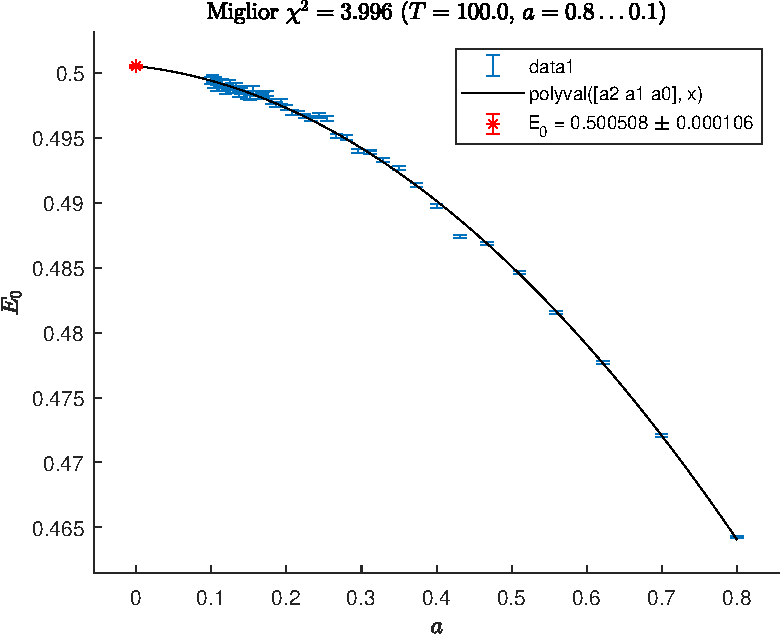
\includegraphics{../plots/qho/final/extrap_E0_fit-crop.pdf}
  \caption{Estrapolazione di $E_0$ per $a=0$. Il miglior polinomio è $a_2 x^2 + a_1 x + a_0$.}
\end{figure}

\begin{figure}[H]
  \centering
  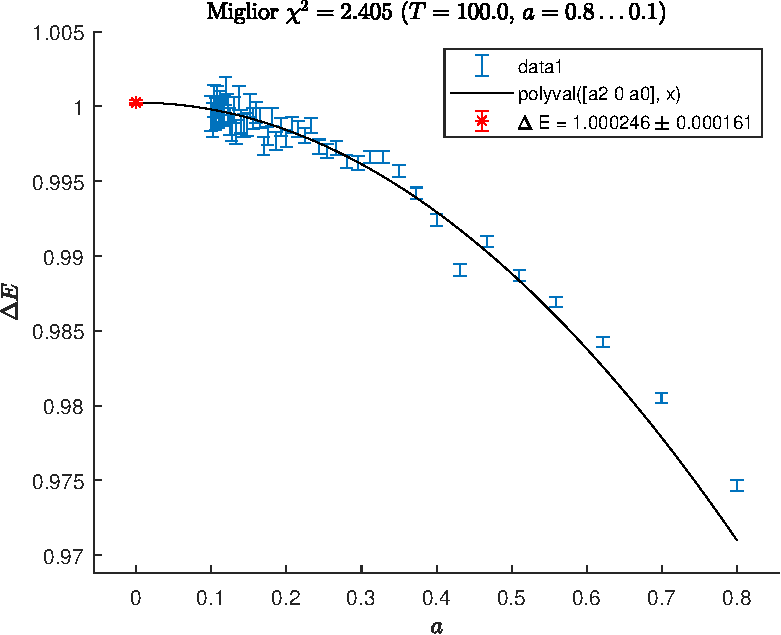
\includegraphics{../plots/qho/final/extrap_DeltaE_fit-crop.pdf}
  \caption{Estrapolazione di $\Delta E$ per $a=0$. Il miglior polinomio è $a_2 x^2 + a_0$.}
\end{figure}

Le stime numeriche ottenute sono soddisfacenti. Si noti che i valori teorici non rientrano negli intervalli definiti dalle incertezze calcolate.
Questo può essere dovuto a due effetti. Innanzitutto le medie che calcoliamo non coincidono esattamente con la proiezione sul vuoto, dato che ci siamo limitati ad un valore fissato di $T$.
Inoltre, la strategia che utilizziamo per l'estrapolazione è empirica, quindi non abbiamo ragione di credere che l'andamento delle stime segua esattamente il polinomio scelto.

Per avere una prima idea della qualità del metodo delineato da Creutz, lo applichiamo anche in questo caso.

\begin{figure}[H]
  \centering
  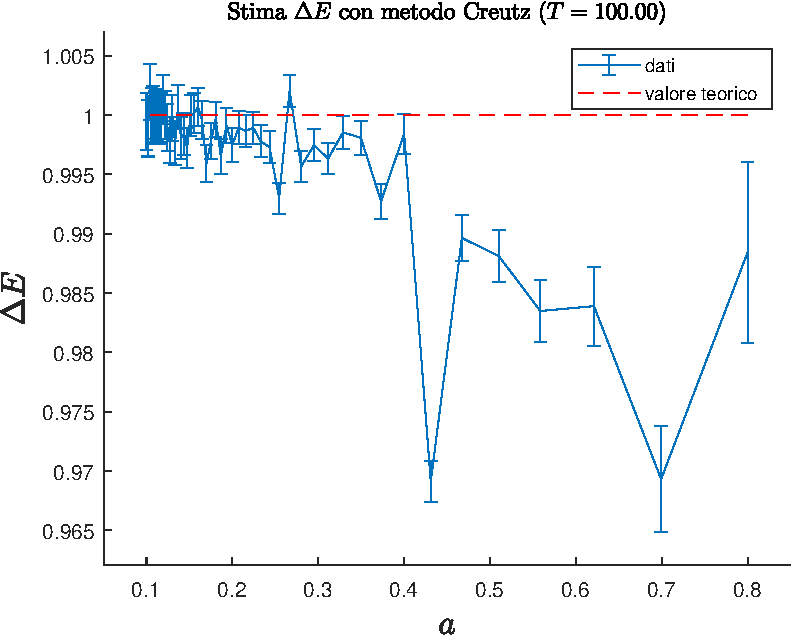
\includegraphics{../plots/qho/final/de_creutz_a0.80-0.10_T100-crop.pdf}
  \caption{}
\end{figure}

Gli errori riportati sono stati ottenuti applicando la propagazione degli errori alla formula \eqref{creutz}.
Inoltre le stime ottenute dalla \eqref{creutz} per vari valori di $\tau$ e $\Delta \tau$ sono state mediate tra loro.
Effettivamente notiamo che per i valori di $a$ più piccoli le stime numeriche sono perfettamente compatibili con il valore teorico.

\subsection{Oscillatore anarmonico quantistico}

Nel caso dell'oscillatore anarmonico non abbiamo direttamente dei valori teorici con cui confrontare le stime numeriche.
Possiamo però fare affidamento alla teoria delle perturbazioni e ottenere comunque un valore approssimato, a patto di mantenere $\lambda$ piccolo e limitarci al caso di $x_0 = 0$.
La perturbazione diventa allora $\lambda H' = \lambda \hat{x}^4$.

Ci serve innanzitutto calcolare la matrice $\Braket{m | H' | n} = \Braket{m | \hat{x}^4 | n}$. Possiamo riscrivere l'operatore di posizione
in termini degli operatori di scala, ma andiamo incontro a conti un po' laboriosi.
Possiamo ricorrere a strumenti di calcolo simbolico, che ne automatizzano il calcolo. A tale scopo è stato utilizzato il modulo python \texttt{sympy}, che include strumenti per i calcoli quantistici.
La forma esplicita della matrice è la seguente, assumendo $m = \omega = \hbar = 1$:

\begin{equation}
  \begin{split}
    & \Braket{m | \hat{x}^4 | n} = \Braket{m | \frac{1}{4} \left(a + a^\dagger\right)^4 | n} = \\
    & = \frac{1}{4} \sqrt{n} \sqrt{n - 3} \sqrt{n - 2} \sqrt{n - 1}\, \delta_{m, n - 4} \\
    & + \left(n \sqrt{n} \sqrt{n - 1} - \frac{1}{2} \sqrt{n} \sqrt{n - 1}\right) \delta_{m, n - 2} \\
    & + \frac{3}{2} \left(n^{2} + n + \frac{1}{2}\right) \delta_{m n} \\
    & + \left(n \sqrt{n + 1} \sqrt{n + 2} + \frac{3}{2} \sqrt{n + 1} \sqrt{n + 2}\right) \delta_{m, n + 2}  \\
    & + \frac{1}{4} \sqrt{n + 1} \sqrt{n + 2} \sqrt{n + 3} \sqrt{n + 4}\, \delta_{m, n + 4} \\
  \end{split}
\end{equation}


Ora siamo in grado di stimare le correzioni previste dalla teoria delle perturbazioni.
Ci limitiamo a considerare le correzioni fino al secondo ordine, dato che correzioni di ordine maggiore diventano più laboriose e danno un contributo di scarsa entità.
Sempre assumendo $m = \omega = 1$, per $\lambda = 0.01$ si ottengono i valori delle energie $E_0 = 0.5072583125$, $E_1 = 1.5356821875$ e $\Delta E = 1.028423875$.

Si riportano i risultati numerici ottenuti con il medesimo valore di $\lambda$.

\begin{figure}[H]
  \centering
  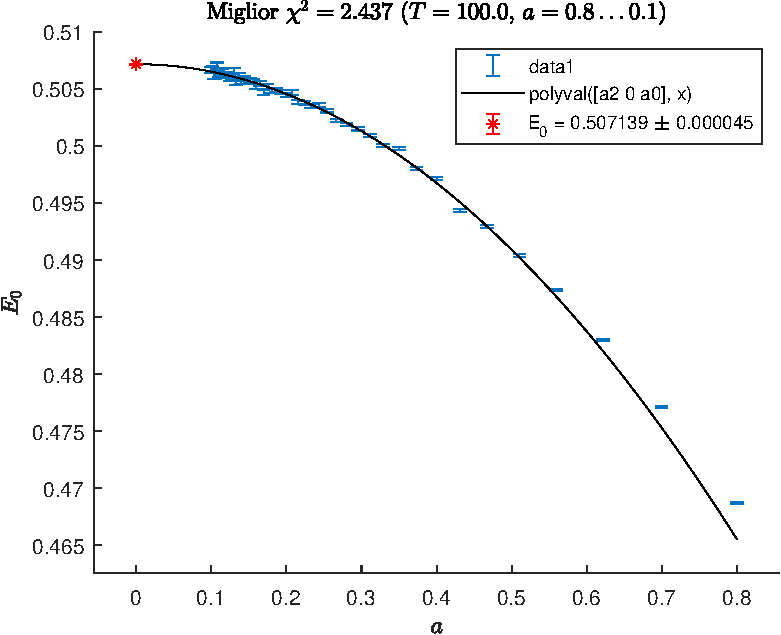
\includegraphics{../plots/qao/final/extrap_E0_fit-crop.pdf}
  \caption{Estrapolazione di $E_0$ per $a=0$. Il miglior polinomio è $a_2 x^2 + a_0$.}
\end{figure}

\begin{figure}[H]
  \centering
  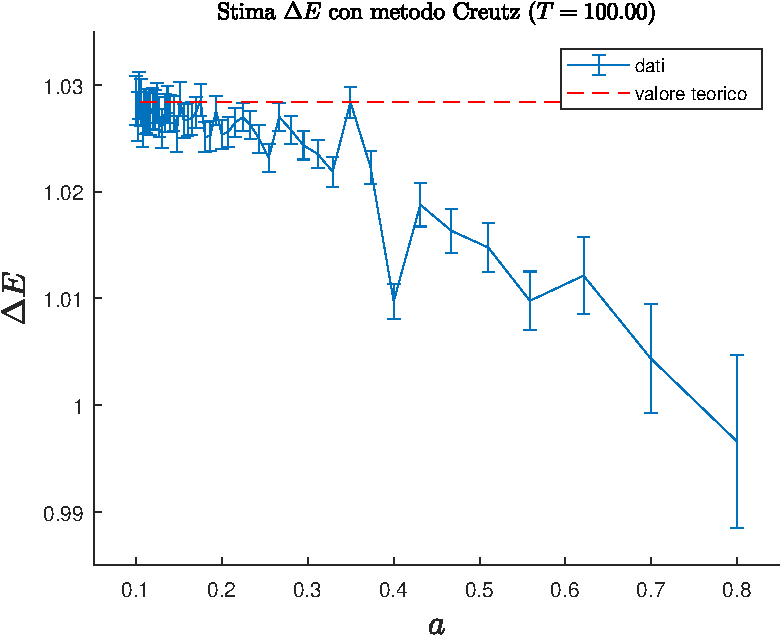
\includegraphics{../plots/qao/final/de_creutz_a0.80-0.10_T100-crop.pdf}
  \caption{Stime di $\Delta E$, calcolate con il metodo di Creutz, al variare di $a$.}
\end{figure}

Anche per l'oscillatore anarmonico valgono le considerazioni fatte nel caso precedente.

Siccome l'andamento delle stime di $\Delta E$ con il metodo Creutz ha un aspetto che ricorda i casi precedenti, si è tentato di
trovare un polinomio adatto con lo stesso metodo già descritto.

\begin{figure}[H]
  \centering
  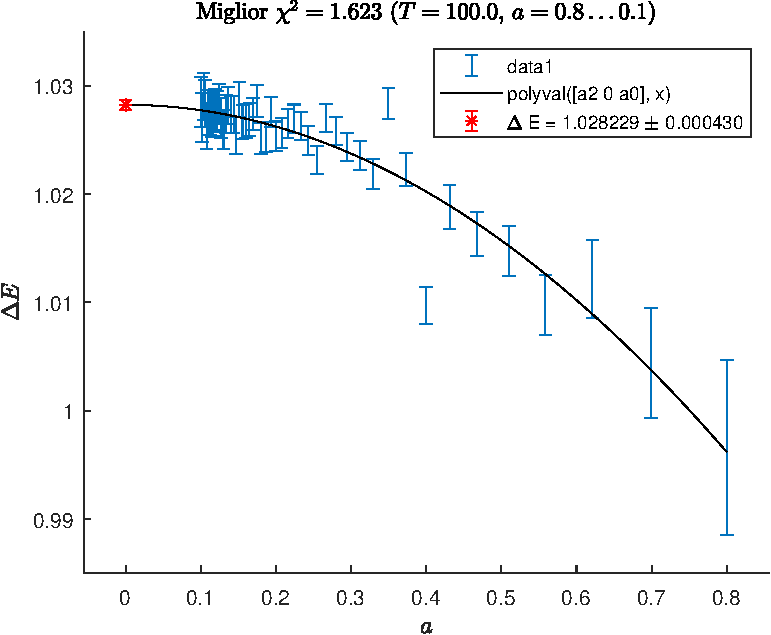
\includegraphics{../plots/qao/final/extrap_DeltaE_creutz_fit-crop.pdf}
  \caption{Estrapolazione di $\Delta E$ per $a=0$. Il miglior polinomio è $a_2 x^2 + a_0$}
\end{figure}


Per pura curiosità, vengono riportati i risultati che si ottengono applicando l'approccio usato per l'oscillatore armonico, dove si assume che l'andamento della correlazione decresca come un singolo esponenziale, ma che sappiamo essere falso.

\begin{figure}[H]
  \centering
  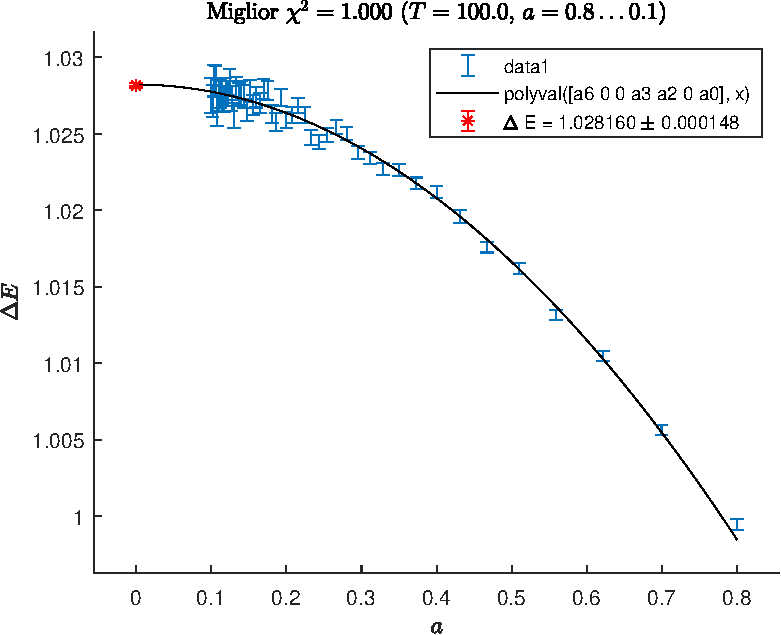
\includegraphics{../plots/qao/final/extrap_DeltaE_fit-crop.pdf}
  \caption{Estrapolazione di $\Delta E$ con il metodo (errato) usato per l'oscillatore armonico. Il miglior polinomio è $a_6 x^6 + a_3 x^3 + a_2 x^2 + a_0$.}
\end{figure}

Anche con questo metodo il risultato non è lontano dal valore teorico. Presumibilmente si tratta di una conseguenza del piccolo valore di $\lambda$ scelto.
Allo stesso tempo però notiamo che il grado del polinomio identificato coincide con il grado massimo per cui avviene la ricerca, che testimonia l'inadeguatezza di questo approccio.

\subsubsection{Distribuzione dei cammini}
Infine si riporta un grafico che mostra la distribuzione dei cammini campionati per l'oscillatore anarmonico.
Per rendere evidente la presenza del termine quartico si è scelto un valore di $x_0$ non nullo. In questo modo la distribuzione diventa bimodale.
In più, per accentuare l'effetto del termine quartico il valore di $\lambda$ è stato incrementato rispetto a prima ($\lambda = 1$).
La linea rossa è la densità di probabilità stimata con il metodo di \emph{kernel density estimation} (KDE), accessibile in MATLAB grazie alla funzione \texttt{kde}.
Questa densità rappresenta una ricostruzione della funzione d'onda (più precisamente del suo modulo quadro) che viene campionata.


\begin{figure}[H]
  \centering
  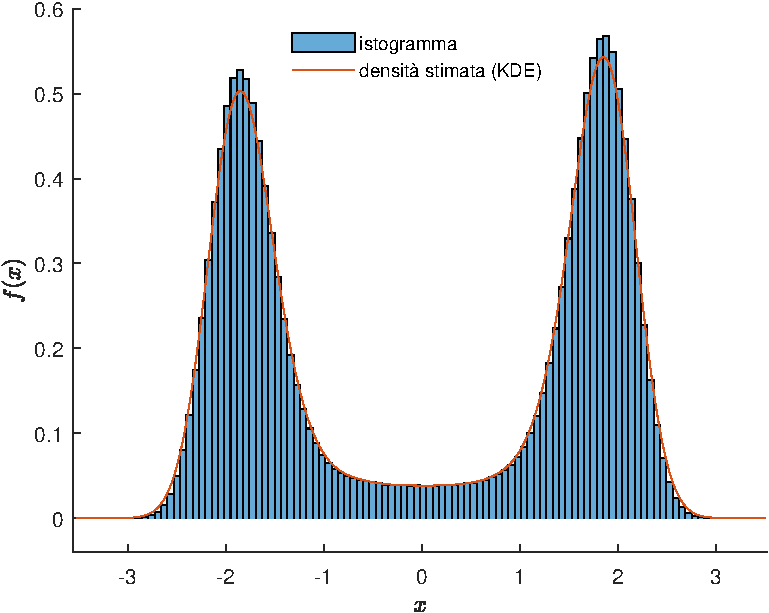
\includegraphics{../plots/qao/final/distr_plot-crop.pdf}
  \caption{Istogramma normalizzato dei cammini campionati. I parametri usati sono $\lambda = 1$, $x_0 = 2$ $a = 0.1$, $T=100$ ($N=1000$).}
\end{figure}


\printbibliography

\end{document}